\documentclass[8pt]{beamer}
\usetheme{Madrid}
\usecolortheme{default}
\usepackage{amsmath, amssymb, graphicx, array, multirow, booktabs, xcolor, tikz}
\usetikzlibrary{shapes,arrows,positioning,fit,backgrounds}

% Compact font settings for tutorial format
\setbeamerfont{title}{size=\Large}
\setbeamerfont{subtitle}{size=\small}
\setbeamerfont{author}{size=\scriptsize}
\setbeamerfont{date}{size=\scriptsize}
\setbeamerfont{frametitle}{size=\large}
\setbeamerfont{framesubtitle}{size=\normalsize}
\setbeamerfont{enumerate item}{size=\footnotesize}
\setbeamerfont{itemize item}{size=\footnotesize}

% Compact spacing
\setlength{\itemsep}{0.08ex}
\setlength{\parskip}{0.08ex}
\setlength{\leftmargini}{0.3cm}
\setbeamersize{text margin left=3mm, text margin right=3mm}
\addtobeamertemplate{frame begin}{\vspace{-0.4cm}}{}

% Colors for tutorial
\definecolor{blue}{RGB}{0,0,255}
\definecolor{red}{RGB}{255,0,0}
\definecolor{green}{RGB}{0,128,0}
\definecolor{orange}{RGB}{255,165,0}
\definecolor{purple}{RGB}{128,0,128}
\definecolor{gray}{RGB}{128,128,128}
\definecolor{lightblue}{RGB}{173,216,230}
\definecolor{lightyellow}{RGB}{255,255,224}
\definecolor{lightgreen}{RGB}{144,238,144}
\definecolor{lightred}{RGB}{255,182,193}

\title{Supervised Learning - Part 2}
\subtitle{COMPLETE TUTORIAL: Decision Trees, KNN, SVM, Neural Networks \& Autoencoders}
\author{GARP RAI Exam Preparation}
\date{}

\begin{document}
	
	\begin{frame}
		\titlepage
	\end{frame}
	
	% ============================================================
	% TUTORIAL INTRODUCTION
	% ============================================================
	
	\begin{frame}{TUTORIAL OVERVIEW}
		\fontsize{7}{8}\selectfont
		\textbf{What You Will Learn in This Tutorial:}
		
		\vspace{0.2cm}
		\begin{tabular}{|p{2.5cm}|p{5.5cm}|}
			\hline
			\textcolor{blue}{Topic} & \textcolor{blue}{Key Concepts Covered} \\
			\hline
			1. Decision Trees & CART, RSS, Entropy, Gini, Pruning, Ensemble Methods \\
			\hline
			2. K-Nearest Neighbors & Lazy Learner, Distance Metrics, K Selection, Curse of Dimensionality \\
			\hline
			3. Support Vector Machines & Margin, Support Vectors, Kernel Trick, Soft Margin \\
			\hline
			4. Neural Networks & MLP, Activation Functions, Backpropagation, Overfitting \\
			\hline
			5. Autoencoders & Encoder-Decoder, Dimensionality Reduction, Anomaly Detection \\
			\hline
		\end{tabular}
		
		\vspace{0.2cm}
		\textbf{Tutorial Format:}
		\begin{itemize}
			\item Each topic presented with \textcolor{blue}{theory}, \textcolor{blue}{mathematics}, \textcolor{blue}{examples}, and \textcolor{blue}{exam traps}
			\item Step-by-step explanations with visual descriptions
			\item Practical tips for risk management applications
		\end{itemize}
		
		\textcolor{red}{\textbf{Key to Success:}} Understand the \textcolor{blue}{"why"} behind each algorithm, not just the \textcolor{blue}{"how"}.
	\end{frame}
	
	% ============================================================
	% SECTION 1: DECISION TREES - Slides 3-27
	% ============================================================
	
	\begin{frame}{DECISION TREES - Introduction}
		\fontsize{6.5}{7.5}\selectfont
		\textcolor{blue}{\textbf{What is a Decision Tree?}}
		
		\begin{itemize}
			\item A \textcolor{blue}{supervised} machine learning technique
			\item Uses a \textcolor{blue}{tree-like structure} for predictions
			\item \textcolor{blue}{Sequentially splits} data based on feature values
			\item Can handle both \textcolor{blue}{classification} and \textcolor{blue}{regression} (CART)
		\end{itemize}
		
		\textbf{Anatomy of a Decision Tree:}
		
		\begin{center}
			\resizebox{0.7\textwidth}{!}{%
				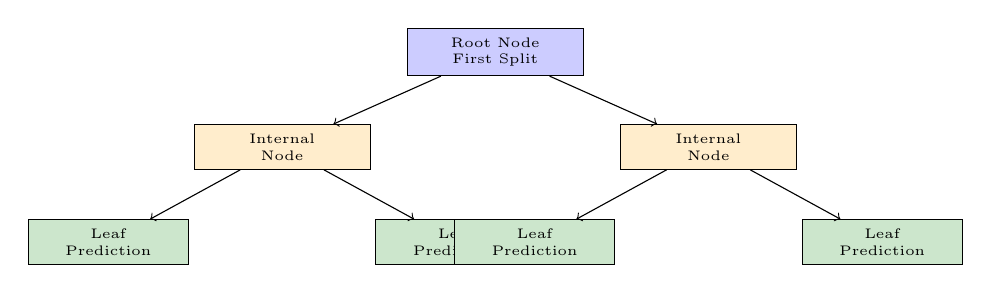
\begin{tikzpicture}[every node/.style={font=\tiny}]
					\node[draw, rectangle, fill=blue!20, text width=2cm, align=center] (root) {Root Node\\First Split};
					\node[draw, rectangle, fill=orange!20, text width=2cm, align=center] (int1) [below left of=root, xshift=-2cm, yshift=-0.5cm] {Internal\\Node};
					\node[draw, rectangle, fill=orange!20, text width=2cm, align=center] (int2) [below right of=root, xshift=2cm, yshift=-0.5cm] {Internal\\Node};
					\node[draw, rectangle, fill=green!20, text width=1.8cm, align=center] (leaf1) [below left of=int1, xshift=-1.5cm, yshift=-0.5cm] {Leaf\\Prediction};
					\node[draw, rectangle, fill=green!20, text width=1.8cm, align=center] (leaf2) [below right of=int1, xshift=1.5cm, yshift=-0.5cm] {Leaf\\Prediction};
					\node[draw, rectangle, fill=green!20, text width=1.8cm, align=center] (leaf3) [below left of=int2, xshift=-1.5cm, yshift=-0.5cm] {Leaf\\Prediction};
					\node[draw, rectangle, fill=green!20, text width=1.8cm, align=center] (leaf4) [below right of=int2, xshift=1.5cm, yshift=-0.5cm] {Leaf\\Prediction};
					\draw[->] (root) -- (int1);
					\draw[->] (root) -- (int2);
					\draw[->] (int1) -- (leaf1);
					\draw[->] (int1) -- (leaf2);
					\draw[->] (int2) -- (leaf3);
					\draw[->] (int2) -- (leaf4);
				\end{tikzpicture}%
			}
		\end{center}
		
		\textcolor{blue}{\textbf{Key Insight:}} Decision trees are \textcolor{blue}{"white-box"} models - highly interpretable!
	\end{frame}
	
	\begin{frame}{DECISION TREES - Why "White-Box"?}
		\fontsize{6.5}{7.5}\selectfont
		\textcolor{blue}{\textbf{White-Box vs Black-Box:}}
		
		\begin{tabular}{|p{4.0cm}|p{4.0cm}|}
			\hline
			\textcolor{blue}{White-Box Models} & \textcolor{red}{Black-Box Models} \\
			\hline
			Decision Trees & Neural Networks \\
			\hline
			\textcolor{green}{Easy to understand} & \textcolor{red}{Difficult to interpret} \\
			\hline
			\textcolor{green}{Traceable decisions} & \textcolor{red}{Hidden decision process} \\
			\hline
			\textcolor{green}{Visual representation} & \textcolor{red}{Complex mathematics} \\
			\hline
			\textcolor{green}{Regulatory friendly} & \textcolor{red}{Regulatory challenges} \\
			\hline
		\end{tabular}
		
		\textbf{Example - Credit Decision:}
		\begin{itemize}
			\item Tree: "Is credit score $>$ 700?" $\rightarrow$ "Is income $>$ \$80,000?" $\rightarrow$ Default Probability = 2\%
			\item \textcolor{green}{Easy to explain to regulators!}
		\end{itemize}
		
		\textcolor{red}{\textbf{Exam Trap:}} Interpretability vs Accuracy trade-off - ensembles improve accuracy but reduce interpretability.
	\end{frame}
	
	\begin{frame}{DECISION TREES - Regression Trees}
		\fontsize{6.5}{7.5}\selectfont
		\textcolor{blue}{\textbf{Regression Trees - For Continuous Target Variables}}
		
		\textbf{Example:} Predicting house price per square foot using:
		\begin{itemize}
			\item Feature 1: Age of house
			\item Feature 2: Distance to metro station
		\end{itemize}
		
		\textbf{How They Work:}
		\begin{enumerate}
			\item Partition feature space into \textcolor{blue}{non-overlapping regions}
			\item Prediction = \textcolor{blue}{average} of training observations in that region
			\item Split criterion: \textcolor{blue}{Minimize RSS}
		\end{enumerate}
		
		\textbf{Key Formula - Residual Sum of Squares (RSS):}
		\[
		RSS = \sum_{j=1}^J \sum_{i \in R_j} (y_i - \bar{y}_{R_j})^2
		\]
		where $\bar{y}_{R_j}$ = mean of observations in region $j$
		
		\textcolor{red}{\textbf{Exam Trap:}} The value that minimizes RSS in a region is the \textcolor{blue}{MEAN}, not the median or mode!
	\end{frame}
	
	\begin{frame}{DECISION TREES - Regression Trees Example}
		\fontsize{6.5}{7.5}\selectfont
		\textcolor{blue}{\textbf{House Price Prediction Example:}}
		
		\textbf{Step 1:} Find first split - Distance to metro $<$ 826.83 feet?
		
		\textbf{Step 2:} Split left branch - Age $<$ 11.7 years?
		
		\begin{center}
			\resizebox{0.65\textwidth}{!}{%
				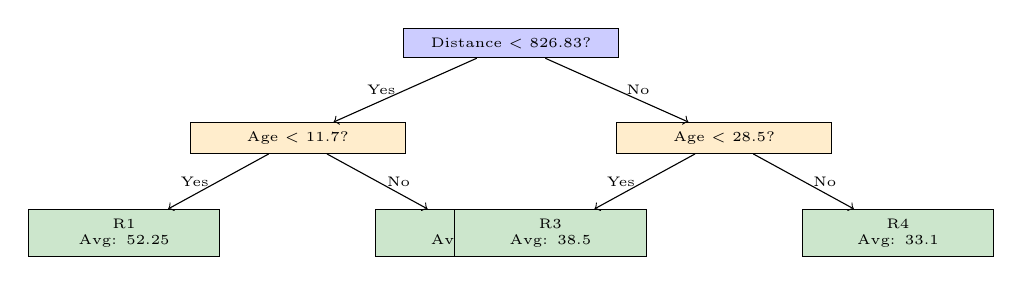
\begin{tikzpicture}[every node/.style={font=\tiny}]
					\node[draw, rectangle, fill=blue!20, text width=2.5cm, align=center] (root) {Distance $<$ 826.83?};
					\node[draw, rectangle, fill=orange!20, text width=2.5cm, align=center] (left) [below left of=root, xshift=-2cm, yshift=-0.5cm] {Age $<$ 11.7?};
					\node[draw, rectangle, fill=orange!20, text width=2.5cm, align=center] (right) [below right of=root, xshift=2cm, yshift=-0.5cm] {Age $<$ 28.5?};
					\node[draw, rectangle, fill=green!20, text width=2.2cm, align=center] (l1) [below left of=left, xshift=-1.5cm, yshift=-0.5cm] {R1\\Avg: 52.25};
					\node[draw, rectangle, fill=green!20, text width=2.2cm, align=center] (l2) [below right of=left, xshift=1.5cm, yshift=-0.5cm] {R2\\Avg: 45.2};
					\node[draw, rectangle, fill=green!20, text width=2.2cm, align=center] (l3) [below left of=right, xshift=-1.5cm, yshift=-0.5cm] {R3\\Avg: 38.5};
					\node[draw, rectangle, fill=green!20, text width=2.2cm, align=center] (l4) [below right of=right, xshift=1.5cm, yshift=-0.5cm] {R4\\Avg: 33.1};
					\draw[->] (root) -- (left) node[midway,left] {Yes};
					\draw[->] (root) -- (right) node[midway,right] {No};
					\draw[->] (left) -- (l1) node[midway,left] {Yes};
					\draw[->] (left) -- (l2) node[midway,right] {No};
					\draw[->] (right) -- (l3) node[midway,left] {Yes};
					\draw[->] (right) -- (l4) node[midway,right] {No};
				\end{tikzpicture}%
			}
		\end{center}
		
		\textbf{Interpretation:}
		\begin{itemize}
			\item \textcolor{blue}{R1:} Close to metro, new houses $\rightarrow$ Highest price (52.25)
			\item \textcolor{blue}{R4:} Far from metro, older houses $\rightarrow$ Lowest price (33.1)
		\end{itemize}
	\end{frame}
	
	\begin{frame}{DECISION TREES - Recursive Binary Splitting}
		\fontsize{6.5}{7.5}\selectfont
		\textcolor{blue}{\textbf{How Trees Are Built - The Algorithm:}}
		
		\textbf{Why Not Try All Possibilities?}
		\begin{itemize}
			\item Number of possible tree structures is \textcolor{red}{astronomical}
			\item Computationally \textcolor{red}{infeasible} for any real dataset
			\item Need a \textcolor{blue}{pragmatic approach}
		\end{itemize}
		
		\textbf{Recursive Binary Splitting:}
		\begin{enumerate}
			\item Start with \textcolor{blue}{all data} in one region (root)
			\item Search every feature and every split point
			\item Find split that \textcolor{blue}{maximizes RSS reduction} (regression) or \textcolor{blue}{maximizes purity} (classification)
			\item Split data into two regions
			\item \textcolor{blue}{Repeat} independently on each region
			\item Stop when \textcolor{blue}{stopping criterion} is met
		\end{enumerate}
		
		\textbf{Stopping Criteria:}
		\begin{itemize}
			\item Minimum observations per leaf
			\item Maximum tree depth
			\item Maximum number of leaves
			\item Minimum information gain
		\end{itemize}
		
		\textcolor{red}{\textbf{Exam Trap:}} This is a \textcolor{blue}{"greedy"} algorithm - it makes locally optimal choices, not globally optimal ones!
	\end{frame}
	
	\begin{frame}{DECISION TREES - Classification Trees}
		\fontsize{6.5}{7.5}\selectfont
		\textcolor{blue}{\textbf{Classification Trees - For Categorical Target Variables}}
		
		\textbf{Example:} Predicting whether a firm will pay dividends
		
		\textbf{Key Difference from Regression Trees:}
		\begin{itemize}
			\item Goal: \textcolor{blue}{Assign observations to a class}
			\item Splitting criterion: \textcolor{blue}{Maximize node purity}
			\item Measures of impurity: \textcolor{blue}{Entropy} or \textcolor{blue}{Gini Coefficient}
		\end{itemize}
		
		\textbf{Entropy Formula:}
		\[
		Entropy = -\sum_{j=1}^J p_j \log_2(p_j)
		\]
		
		\textbf{Gini Coefficient Formula:}
		\[
		Gini = 1 - \sum_{j=1}^J p_j^2
		\]
		
		\textbf{Interpretation:}
		\begin{itemize}
			\item \textcolor{green}{Lower values} = more pure nodes
			\item \textcolor{green}{Perfect purity} = all observations in one class $\rightarrow$ Entropy = 0, Gini = 0
			\item \textcolor{red}{Maximum impurity} = equal class distribution $\rightarrow$ Entropy = 1 (binary), Gini = 0.5 (binary)
		\end{itemize}
		
		\textcolor{red}{\textbf{Exam Trap:}} Entropy and Gini usually lead to \textcolor{blue}{similar trees} - don't overthink the choice!
	\end{frame}
	
	\begin{frame}{DECISION TREES - Entropy Calculation Example}
		\fontsize{6.5}{7.5}\selectfont
		\textcolor{blue}{\textbf{Entropy - Worked Example:}}
		
		\textbf{Scenario:} Node with 100 observations: 70 Non-Default, 30 Default
		
		\textbf{Step 1:} Calculate probabilities:
		\begin{itemize}
			\item $p_{\text{Non-Default}} = 70/100 = 0.7$
			\item $p_{\text{Default}} = 30/100 = 0.3$
		\end{itemize}
		
		\textbf{Step 2:} Apply entropy formula:
		\[
		Entropy = -[0.7 \log_2(0.7) + 0.3 \log_2(0.3)]
		\]
		
		\textbf{Step 3:} Calculate:
		\begin{itemize}
			\item $\log_2(0.7) \approx -0.5146$
			\item $\log_2(0.3) \approx -1.7370$
			\item Entropy = $-[0.7 \times (-0.5146) + 0.3 \times (-1.7370)]$
			\item Entropy = $-[-0.3602 - 0.5211] = 0.8813$
		\end{itemize}
		
		\textbf{Interpretation:}
		\begin{itemize}
			\item Entropy ranges from \textcolor{green}{0} (pure) to \textcolor{red}{1} (maximum impurity for binary)
			\item 0.8813 indicates \textcolor{orange}{moderate impurity}
			\item Not a perfect split, but better than 50-50
		\end{itemize}
	\end{frame}
	
	\begin{frame}{DECISION TREES - Gini Calculation Example}
		\fontsize{6.5}{7.5}\selectfont
		\textcolor{blue}{\textbf{Gini Coefficient - Worked Example:}}
		
		\textbf{Same Scenario:} Node with 100 observations: 70 Non-Default, 30 Default
		
		\textbf{Step 1:} Calculate probabilities:
		\begin{itemize}
			\item $p_{\text{Non-Default}} = 0.7$
			\item $p_{\text{Default}} = 0.3$
		\end{itemize}
		
		\textbf{Step 2:} Apply Gini formula:
		\[
		Gini = 1 - (0.7^2 + 0.3^2)
		\]
		
		\textbf{Step 3:} Calculate:
		\begin{itemize}
			\item $0.7^2 = 0.49$
			\item $0.3^2 = 0.09$
			\item Sum = $0.49 + 0.09 = 0.58$
			\item Gini = $1 - 0.58 = 0.42$
		\end{itemize}
		
		\textbf{Comparison Table:}
		
		\begin{tabular}{|p{3cm}|p{3cm}|p{3cm}|}
			\hline
			\textbf{Node Distribution} & \textbf{Entropy} & \textbf{Gini} \\
			\hline
			100\% Pure (70-0 or 0-70) & 0 & 0 \\
			\hline
			80-20 split & 0.722 & 0.32 \\
			\hline
			70-30 split & 0.881 & 0.42 \\
			\hline
			50-50 split & 1.0 & 0.5 \\
			\hline
		\end{tabular}
		
		\textcolor{red}{\textbf{Exam Trap:}} Both measures \textcolor{blue}{decrease as purity increases} - they give similar results!
	\end{frame}
	
	\begin{frame}{DECISION TREES - Information Gain}
		\fontsize{6.5}{7.5}\selectfont
		\textcolor{blue}{\textbf{Information Gain - Selecting the Best Split}}
		
		\textbf{What is Information Gain?}
		\begin{itemize}
			\item The \textcolor{blue}{reduction in impurity} achieved by a split
			\item Formula: $\text{IG} = \text{Parent Impurity} - \text{Weighted Child Impurities}$
		\end{itemize}
		
		\textbf{Dividend Payment Example:}
		
		\textbf{Step 1:} Baseline Gini = 0.480 (no split)
		
		\textbf{Step 2:} Split on "Large\_Cap":
		\begin{itemize}
			\item Large Cap (13 firms): 11 paid, 2 not $\rightarrow$ Gini = 0.260
			\item Non-Large Cap (7 firms): 1 paid, 6 not $\rightarrow$ Gini = 0.245
			\item Weighted Gini = $(13/20 \times 0.260) + (7/20 \times 0.245) = 0.255$
		\end{itemize}
		
		\textbf{Step 3:} Calculate Information Gain:
		\[
		IG = 0.480 - 0.255 = 0.225
		\]
		
		\textbf{Step 4:} Repeat for all features $\rightarrow$ Choose feature with \textcolor{blue}{highest IG}
		
		\textcolor{red}{\textbf{Exam Trap:}} Information gain is \textcolor{blue}{ALWAYS $\geq$ 0}! A good split reduces impurity.
	\end{frame}
	
	\begin{frame}{DECISION TREES - Continuous Feature Splitting}
		\fontsize{6.5}{7.5}\selectfont
		\textcolor{blue}{\textbf{Handling Continuous Features in Decision Trees}}
		
		\textbf{The Challenge:}
		\begin{itemize}
			\item Continuous features can take \textcolor{blue}{any value} (e.g., Retail\_Investor = 0-100\%)
			\item Need to find the \textcolor{blue}{optimal threshold} for splitting
		\end{itemize}
		
		\textbf{Algorithm:}
		\begin{enumerate}
			\item Sort the continuous feature values
			\item Consider each distinct value as a \textcolor{blue}{potential threshold}
			\item Calculate information gain for \textcolor{blue}{each} threshold
			\item Select the threshold that \textcolor{blue}{maximizes} information gain
		\end{enumerate}
		
		\textbf{Example - Retail\_Investor:}
		\begin{itemize}
			\item Values: 20\%, 30\%, 40\%, 50\%, 60\%, 70\%, 80\%
			\item Test threshold: 35\% $\rightarrow$ Left: $\leq$ 35\%, Right: $>$ 35\%
			\item Test threshold: 45\% $\rightarrow$ Left: $\leq$ 45\%, Right: $>$ 45\%
			\item Choose the threshold with \textcolor{blue}{highest information gain}
		\end{itemize}
		
		\textbf{Key Insight:}
		\begin{itemize}
			\item This is an \textcolor{blue}{automated} process in machine learning packages
			\item The optimal threshold depends on the \textcolor{blue}{node} (not fixed globally!)
		\end{itemize}
	\end{frame}
	
	\begin{frame}{DECISION TREES - Pruning}
		\fontsize{6.5}{7.5}\selectfont
		\textcolor{blue}{\textbf{Pruning - Reducing Tree Complexity}}
		
		\textbf{Why Prune?}
		\begin{enumerate}
			\item \textcolor{blue}{Prevent overfitting}
			\item \textcolor{blue}{Improve interpretability}
			\item \textcolor{blue}{Remove irrelevant features}
		\end{enumerate}
		
		\textbf{Two Types of Pruning:}
		
		\begin{tabular}{|p{4cm}|p{4cm}|}
			\hline
			\textcolor{blue}{Pre-Pruning (Online)} & \textcolor{blue}{Post-Pruning (Offline)} \\
			\hline
			During tree growth & After tree is fully grown \\
			\hline
			Stopping criteria & Remove weak links \\
			\hline
			Minimum leaf size & Reduced error pruning \\
			\hline
			Maximum depth & Cost-complexity pruning \\
			\hline
			Minimum information gain & Bottom-up approach \\
			\hline
			\textcolor{green}{Computationally efficient} & \textcolor{orange}{More computationally intensive} \\
			\hline
		\end{tabular}
		
		\textbf{Reduced Error Pruning:}
		\begin{enumerate}
			\item Start at \textcolor{blue}{leaves} (bottom-up)
			\item Replace a node with its \textcolor{blue}{most popular class}
			\item Accept if \textcolor{blue}{validation performance doesn't degrade}
		\end{enumerate}
		
		\textcolor{red}{\textbf{Exam Trap:}} Post-pruning often finds \textcolor{blue}{better trees} but is more computationally expensive!
	\end{frame}
	
	\begin{frame}{DECISION TREES - Cost-Complexity Pruning}
		\fontsize{6.5}{7.5}\selectfont
		\textcolor{blue}{\textbf{Cost-Complexity Pruning - Mathematical Formulation}}
		
		\textbf{Objective Function:}
		\[
		\text{Minimize } RSS + \alpha \times (\text{Number of Leaves})
		\]
		
		\textbf{Components:}
		\begin{itemize}
			\item $RSS$: Residual Sum of Squares (fit to training data)
			\item $\alpha$: \textcolor{blue}{Complexity parameter} (tuning parameter)
			\item Number of Leaves: Model complexity
		\end{itemize}
		
		\textbf{Effect of $\alpha$:}
		\begin{itemize}
			\item $\alpha = 0$: No penalty $\rightarrow$ \textcolor{red}{Largest tree} (overfit)
			\item $\alpha$ very large: Heavy penalty $\rightarrow$ \textcolor{red}{Smallest tree} (underfit)
			\item Optimal $\alpha$: \textcolor{green}{Best balance} of fit and complexity
		\end{itemize}
		
		\textbf{Selecting $\alpha$:}
		\begin{enumerate}
			\item Define a grid of $\alpha$ values
			\item For each $\alpha$, build and prune a tree
			\item Use \textcolor{blue}{cross-validation} to select best $\alpha$
			\item Choose $\alpha$ that minimizes validation error
		\end{enumerate}
		
		\textcolor{red}{\textbf{Exam Trap:}} Cross-validation is the \textcolor{blue}{standard method} for selecting $\alpha$ - not arbitrary choice!
	\end{frame}
	
	\begin{frame}{DECISION TREES - Bagging}
		\fontsize{6.5}{7.5}\selectfont
		\textcolor{blue}{\textbf{Ensemble Method 1: Bagging (Bootstrap Aggregation)}}
		
		\textbf{Core Idea:}
		\begin{itemize}
			\item Create \textcolor{blue}{multiple} decision trees
			\item Each tree trained on a \textcolor{blue}{different bootstrap sample}
			\item Aggregate predictions
		\end{itemize}
		
		\textbf{Algorithm:}
		\begin{enumerate}
			\item Sample with replacement (\textcolor{blue}{bootstrapping}) from training data
			\item Train a decision tree on each sample
			\item Repeat many times (e.g., 500 trees)
			\item Aggregation: \textcolor{blue}{Average} (regression) or \textcolor{blue}{Majority Vote} (classification)
		\end{enumerate}
		
		\textbf{Example:}
		\begin{itemize}
			\item Training set: 100,000 observations
			\item Each bootstrap sample: 10,000 observations (with replacement)
			\item About \textcolor{blue}{63.2\%} of observations appear in each sample
			\item \textcolor{blue}{36.8\%} are \textcolor{blue}{Out-of-Bag (OOB)} - used for validation
		\end{itemize}
		
		\textbf{Why It Works:}
		\begin{itemize}
			\item Reduces \textcolor{blue}{variance} by averaging models
			\item If models are uncorrelated: $Var(\bar{Y}) = Var(Y)/M$
		\end{itemize}
	\end{frame}
	
	\begin{frame}{DECISION TREES - Random Forests}
		\fontsize{6.5}{7.5}\selectfont
		\textcolor{blue}{\textbf{Ensemble Method 2: Random Forests}}
		
		\textbf{Improvement Over Bagging:}
		\begin{itemize}
			\item Same as bagging \textcolor{blue}{PLUS} feature randomization
			\item At each split, consider only a \textcolor{blue}{random subset} of features
			\item Typical: $\sqrt{p}$ features where $p$ = total features
		\end{itemize}
		
		\textbf{Why Feature Randomization?}
		\begin{itemize}
			\item Bagging trees can be \textcolor{red}{highly correlated}
			\item If a feature is very strong, it appears in \textcolor{red}{all} trees
			\item Correlation $\rightarrow$ less benefit from averaging
			\item Random forests $\rightarrow$ \textcolor{blue}{de-correlated} trees
		\end{itemize}
		
		\textbf{Comparison:}
		
		\begin{tabular}{|p{3cm}|p{3cm}|p{3cm}|}
			\hline
			\textbf{Feature} & \textbf{Bagging} & \textbf{Random Forest} \\
			\hline
			Feature subset & All features & $\sqrt{p}$ features \\
			\hline
			Tree correlation & High & Low \\
			\hline
			Variance reduction & Moderate & \textcolor{green}{High} \\
			\hline
		\end{tabular}
		
		\textcolor{red}{\textbf{Exam Trap:}} Random forests sacrifice individual tree optimality for \textcolor{blue}{ensemble diversity}!
	\end{frame}
	
	\begin{frame}{DECISION TREES - Boosting}
		\fontsize{6.5}{7.5}\selectfont
		\textcolor{blue}{\textbf{Ensemble Method 3: Boosting}}
		
		\textbf{Core Idea:}
		\begin{itemize}
			\item Build trees \textcolor{blue}{sequentially}
			\item Each new tree corrects errors of previous trees
		\end{itemize}
		
		\textbf{Gradient Boosting:}
		\begin{enumerate}
			\item Fit a simple tree to the data
			\item Calculate \textcolor{blue}{residuals} (errors)
			\item Fit next tree to the \textcolor{blue}{residuals}
			\item Combine predictions
			\item Repeat, each tree fits residuals of the combined model
		\end{enumerate}
		
		\textbf{AdaBoost:}
		\begin{enumerate}
			\item Start with \textcolor{blue}{equal weights} on all observations
			\item Train a tree
			\item Increase weights of \textcolor{blue}{misclassified} observations
			\item Train next tree with updated weights
			\item Final model: \textcolor{blue}{weighted sum} of trees
		\end{enumerate}
		
		\textcolor{red}{\textbf{Exam Trap:}} Boosting is \textcolor{blue}{sequential} (not parallel) and can \textcolor{red}{overfit} if not carefully tuned!
	\end{frame}
	
	\begin{frame}{DECISION TREES - Boosting vs Bagging Summary}
		\fontsize{6.5}{7.5}\selectfont
		\textcolor{blue}{\textbf{Boosting vs Bagging - Key Differences:}}
		
		\begin{tabular}{|p{3.5cm}|p{3.5cm}|p{3.5cm}|}
			\hline
			\textbf{Aspect} & \textcolor{blue}{Bagging/RF} & \textcolor{blue}{Boosting} \\
			\hline
			Training & \textcolor{green}{Parallel} & \textcolor{red}{Sequential} \\
			\hline
			Focus & Reduce variance & Reduce bias \\
			\hline
			Overfitting Risk & Low & \textcolor{red}{High} \\
			\hline
			Interpretability & Low & Very Low \\
			\hline
			Speed & Fast & Slow \\
			\hline
		\end{tabular}
		
		\textbf{When to Use Each:}
		
		\begin{itemize}
			\item \textcolor{blue}{Bagging/Random Forests:}
			\begin{itemize}
				\item When you have many features
				\item When you want robust performance
				\item When you want to avoid overfitting
			\end{itemize}
			
			\item \textcolor{blue}{Boosting:}
			\begin{itemize}
				\item When you need maximum accuracy
				\item When you have enough data to validate carefully
				\item When you are willing to do extensive hyperparameter tuning
			\end{itemize}
		\end{itemize}
		
		\textcolor{red}{\textbf{Exam Trap:}} Boosting is \textcolor{blue}{more powerful} but \textcolor{red}{more dangerous} (overfitting)!
	\end{frame}
	
	\begin{frame}{DECISION TREES - Practical Considerations}
		\fontsize{6.5}{7.5}\selectfont
		\textcolor{blue}{\textbf{Decision Trees - Practical Tips for Risk Management}}
		
		\textbf{Advantages:}
		\begin{enumerate}
			\item \textcolor{green}{Highly interpretable} - easy to explain to regulators
			\item \textcolor{green}{Handles both continuous and categorical} features
			\item \textcolor{green}{No feature scaling} required
			\item \textcolor{green}{Handles missing values} (in some implementations)
		\end{enumerate}
		
		\textbf{Disadvantages:}
		\begin{enumerate}
			\item \textcolor{red}{Prone to overfitting} (single tree)
			\item \textcolor{red}{Lower accuracy} than more complex models
			\item \textcolor{red}{Unstable} - small data changes can create different trees
			\item \textcolor{red}{Biased toward features with many levels}
		\end{enumerate}
		
		\textbf{Risk Management Applications:}
		\begin{itemize}
			\item Credit scoring (default prediction)
			\item Fraud detection
			\item Operational risk classification
			\item Regulatory capital calculations
		\end{itemize}
		
		\textcolor{red}{\textbf{Exam Trap:}} In risk management, \textcolor{blue}{interpretability} is often as important as \textcolor{blue}{accuracy}!
	\end{frame}
	
	% ============================================================
	% SECTION 2: K-NEAREST NEIGHBORS - Slides 28-40
	% ============================================================
	
	\begin{frame}{KNN - Introduction}
		\fontsize{6.5}{7.5}\selectfont
		\textcolor{blue}{\textbf{K-Nearest Neighbors (KNN) - Overview}}
		
		\textbf{What is KNN?}
		\begin{itemize}
			\item \textcolor{blue}{Supervised} learning algorithm
			\item Used for \textcolor{blue}{classification} and \textcolor{blue}{regression}
			\item \textcolor{blue}{Non-parametric} - no underlying distribution assumed
			\item \textcolor{blue}{Instance-based} - memorizes training data
		\end{itemize}
		
		\textbf{Why "Lazy Learner"?}
		\begin{itemize}
			\item No explicit training phase
			\item Just \textcolor{blue}{stores} the training data
			\item All "work" happens at \textcolor{blue}{prediction time}
		\end{itemize}
		
		\textbf{Core Idea:}
		\begin{itemize}
			\item "Tell me who your neighbors are, and I'll tell you who you are"
			\item For a new instance, find the \textcolor{blue}{K closest} training instances
			\item Classification: \textcolor{blue}{Majority vote} of neighbors
			\item Regression: \textcolor{blue}{Average} of neighbors' values
		\end{itemize}
		
		\textbf{Key Hyperparameters:}
		\begin{enumerate}
			\item \textcolor{blue}{K}: Number of neighbors to consider
			\item \textcolor{blue}{Distance Metric}: How to measure closeness
			\item \textcolor{blue}{Weighting}: Equal or distance-weighted
		\end{enumerate}
	\end{frame}
	
	\begin{frame}{KNN - Distance Metrics}
		\fontsize{6.5}{7.5}\selectfont
		\textcolor{blue}{\textbf{Distance Metrics in KNN}}
		
		\textbf{Euclidean Distance (L2 Norm):}
		\[
		d_E(x, x') = \sqrt{\sum_{j=1}^m (x_j - x'_j)^2}
		\]
		\begin{itemize}
			\item Most common choice
			\item Straight-line distance
			\item Sensitive to scale
		\end{itemize}
		
		\textbf{Manhattan Distance (L1 Norm):}
		\[
		d_M(x, x') = \sum_{j=1}^m |x_j - x'_j|
		\]
		\begin{itemize}
			\item Sum of absolute differences
			\item More robust to outliers
			\item Less sensitive to scale
		\end{itemize}
		
		\textbf{Other Metrics:}
		\begin{itemize}
			\item Cosine similarity (text data)
			\item Minkowski distance (generalization of L1 and L2)
			\item Hamming distance (binary/categorical data)
		\end{itemize}
		
		\textbf{Which to Choose?}
		\begin{itemize}
			\item \textcolor{blue}{Euclidean}: Continuous, well-scaled features
			\item \textcolor{blue}{Manhattan}: High-dimensional data
			\item \textcolor{blue}{Hamming}: Binary/categorical features
		\end{itemize}
		
		\textcolor{red}{\textbf{Exam Trap:}} Choice of distance metric \textcolor{blue}{significantly affects} KNN performance!
	\end{frame}
	
	\begin{frame}{KNN - Feature Scaling}
		\fontsize{6.5}{7.5}\selectfont
		\textcolor{blue}{\textbf{Why Feature Scaling is CRITICAL for KNN}}
		
		\textbf{The Problem:}
		\begin{itemize}
			\item KNN relies on distance calculations
			\item Features with \textcolor{red}{larger scales dominate} the distance
			\item Smaller-scale features become \textcolor{red}{irrelevant}
		\end{itemize}
		
		\textbf{Example - Without Scaling:}
		\begin{tabular}{|p{3cm}|p{3cm}|p{3cm}|}
			\hline
			\textbf{Feature} & \textbf{Range} & \textbf{Scale} \\
			\hline
			Income & \$20,000 - \$500,000 & \textcolor{red}{Large} \\
			\hline
			Age & 18 - 80 & \textcolor{green}{Small} \\
			\hline
		\end{tabular}
		\begin{itemize}
			\item Income dominates distance calculation
			\item Age has almost no effect
			\item \textcolor{red}{Model effectively ignores age!}
		\end{itemize}
		
		\textbf{Solution - Scaling Methods:}
		\begin{enumerate}
			\item \textcolor{blue}{Standardization:} $x' = \frac{x - \mu}{\sigma}$ (mean 0, std 1)
			\item \textcolor{blue}{Min-Max Normalization:} $x' = \frac{x - \min}{\max - \min}$ (range 0 to 1)
		\end{enumerate}
		
		\textcolor{red}{\textbf{Exam Trap:}} \textcolor{blue}{ALWAYS scale features} before applying KNN - it's not optional!
	\end{frame}
	
	\begin{frame}{KNN - Choosing K}
		\fontsize{6.5}{7.5}\selectfont
		\textcolor{blue}{\textbf{How to Choose K in KNN}}
		
		\textbf{Effect of K:}
		
		\begin{tabular}{|p{4cm}|p{4cm}|}
			\hline
			\textcolor{blue}{Small K} & \textcolor{blue}{Large K} \\
			\hline
			More complex model & Simpler model \\
			\hline
			\textcolor{red}{Overfitting} risk & \textcolor{red}{Underfitting} risk \\
			\hline
			Sensitive to noise & Smoother boundaries \\
			\hline
			High variance & High bias \\
			\hline
		\end{tabular}
		
		\textbf{Heuristics:}
		\begin{enumerate}
			\item \textcolor{blue}{$K = \sqrt{N}$} where $N$ = training set size
			\item \textcolor{blue}{$K = \log(N)$} for very large datasets
			\item \textcolor{blue}{Use odd K} to avoid ties in classification
		\end{enumerate}
		
		\textbf{Cross-Validation Method:}
		\begin{enumerate}
			\item Try a range of K values (e.g., 1, 3, 5, 7, ..., 50)
			\item Use cross-validation to estimate test error
			\item Select K with \textcolor{blue}{lowest validation error}
		\end{enumerate}
		
		\textbf{Example:}
		\begin{itemize}
			\item $N = 10,000 \rightarrow K = \sqrt{10,000} = 100$
			\item But cross-validation might suggest K = 85 or K = 120
			\item \textcolor{blue}{Always validate!}
		\end{itemize}
	\end{frame}
	
	\begin{frame}{KNN - Curse of Dimensionality}
		\fontsize{6.5}{7.5}\selectfont
		\textcolor{blue}{\textbf{Curse of Dimensionality in KNN}}
		
		\textbf{The Problem:}
		\begin{itemize}
			\item As the number of features ($m$) increases
			\item Distances become \textcolor{red}{less meaningful}
			\item All points become approximately \textcolor{red}{equidistant}
		\end{itemize}
		
		\textbf{Mathematical Insight:}
		\begin{itemize}
			\item In high dimensions, the \textcolor{blue}{ratio} of distances between nearest and farthest points approaches 1
			\item "Nearest neighbor" loses its meaning
		\end{itemize}
		
		\textbf{Example:}
		\begin{itemize}
			\item 1D space: Points clearly have nearest neighbors
			\item 2D space: Some points are clearly closer
			\item 100D space: All points are about the same distance from each other
		\end{itemize}
		
		\textbf{Mitigation Strategies:}
		\begin{enumerate}
			\item \textcolor{blue}{Feature Selection}: Choose only relevant features
			\item \textcolor{blue}{Dimensionality Reduction}: PCA, Autoencoders
			\item \textcolor{blue}{Specialized Distance Metrics}: For high-dimensional data
			\item \textcolor{blue}{More Data}: Larger training sets help
		\end{enumerate}
		
		\textcolor{red}{\textbf{Exam Trap:}} The curse of dimensionality makes KNN \textcolor{red}{less effective} with many features!
	\end{frame}
	
	\begin{frame}{KNN - Advantages and Disadvantages}
		\fontsize{6.5}{7.5}\selectfont
		\textcolor{blue}{\textbf{KNN - Summary of Pros and Cons}}
		
		\textbf{Advantages:}
		\begin{enumerate}
			\item \textcolor{green}{Simple and intuitive}
			\item \textcolor{green}{No training phase} - fast to "train"
			\item \textcolor{green}{No assumptions} about data distribution
			\item \textcolor{green}{Can handle multi-class} problems
			\item \textcolor{green}{Can handle regression and classification}
			\item \textcolor{green}{Natural for multi-class problems}
		\end{enumerate}
		
		\textbf{Disadvantages:}
		\begin{enumerate}
			\item \textcolor{red}{Computationally expensive for predictions} ($O(N \times m)$)
			\item \textcolor{red}{Sensitive to feature scaling}
			\item \textcolor{red}{Curse of dimensionality}
			\item \textcolor{red}{Sensitive to noise and outliers}
			\item \textcolor{red}{Cannot handle missing values without imputation}
			\item \textcolor{red}{Not interpretable} (no model to explain)
		\end{enumerate}
		
		\textbf{When to Use KNN:}
		\begin{itemize}
			\item Small to medium datasets
			\item Well-scaled, low-dimensional features
			\item When interpretability is not critical
			\item When you need a simple baseline model
		\end{itemize}
		
		\textcolor{red}{\textbf{Exam Trap:}} KNN is \textcolor{blue}{great for small datasets} but \textcolor{red}{struggles with large ones}!
	\end{frame}
	
	\begin{frame}{KNN - Worked Example}
		\fontsize{6.5}{7.5}\selectfont
		\textcolor{blue}{\textbf{KNN Classification - Step-by-Step Example}}
		
		\textbf{Data:} Borrower Default Prediction
		
		\begin{tabular}{|c|c|c|c|}
			\hline
			\textbf{ID} & \textbf{Balance} & \textbf{Income} & \textbf{Default} \\
			\hline
			1 & -0.55 & -0.75 & 0 (No) \\
			\hline
			2 & -0.23 & 0.19 & 0 \\
			\hline
			3 & -0.76 & 0.53 & 0 \\
			\hline
			4 & -0.08 & -0.73 & 0 \\
			\hline
			5 & -0.72 & 1.32 & 0 \\
			\hline
			6 & -0.79 & 2.00 & 0 \\
			\hline
			7 & -0.80 & -0.34 & 0 \\
			\hline
			8 & 0.46 & -0.71 & 1 (Yes) \\
			\hline
			9 & 1.95 & -0.96 & 1 \\
			\hline
			10 & 1.51 & -0.54 & 1 \\
			\hline
		\end{tabular}
		
		\textbf{New Borrower:}
		\begin{itemize}
			\item Balance = 0.90
			\item Income = -0.61
		\end{itemize}
		
		\textbf{Step 1:} Choose K = 4
		
		\textbf{Step 2:} Calculate distances (Euclidean)
		\begin{itemize}
			\item To ID 8: $\sqrt{(0.46-0.90)^2 + (-0.71+0.61)^2} = 0.451$
			\item To ID 10: $\sqrt{(1.51-0.90)^2 + (-0.54+0.61)^2} = 0.611$
			\item To ID 4: $\sqrt{(-0.08-0.90)^2 + (-0.73+0.61)^2} = 0.994$
			\item To ID 9: $\sqrt{(1.95-0.90)^2 + (-0.96+0.61)^2} = 1.105$
		\end{itemize}
		
		\textbf{Step 3:} 4 nearest: 8, 10, 4, 9 (3 Default, 1 Non-Default)
		
		\textbf{Step 4:} Majority vote $\rightarrow$ \textcolor{blue}{Default!}
	\end{frame}
	
	% ============================================================
	% SECTION 3: SUPPORT VECTOR MACHINES - Slides 41-60
	% ============================================================
	
	\begin{frame}{SVM - Introduction}
		\fontsize{6.5}{7.5}\selectfont
		\textcolor{blue}{\textbf{Support Vector Machines (SVM) - Overview}}
		
		\textbf{What is SVM?}
		\begin{itemize}
			\item \textcolor{blue}{Supervised} learning algorithm
			\item Primarily for \textcolor{blue}{classification}
			\item Finds the \textcolor{blue}{optimal separating hyperplane}
			\item Can handle \textcolor{blue}{linear} and \textcolor{blue}{non-linear} boundaries
		\end{itemize}
		
		\textbf{Core Concepts:}
		\begin{enumerate}
			\item \textcolor{blue}{Hyperplane}: Decision boundary
			\item \textcolor{blue}{Margin}: Distance between boundary and closest points
			\item \textcolor{blue}{Support Vectors}: Points that define the margin
		\end{enumerate}
		
		\textbf{Key Idea:}
		\begin{itemize}
			\item Find the hyperplane that \textcolor{blue}{maximizes the margin}
			\item Wider margin $\rightarrow$ \textcolor{blue}{better generalization}
		\end{itemize}
		
		\textbf{SVM Optimization:}
		\[
		\min_{w} \frac{1}{2}|w|^2
		\]
		subject to: $y_j(w_0 + w^T x_j) \geq 1$ for all $j$
		
		\textcolor{red}{\textbf{Exam Trap:}} Maximizing margin $\Leftrightarrow$ Minimizing $|w|$!
	\end{frame}
	
	\begin{frame}{SVM - Mathematical Formulation}
		\fontsize{6.5}{7.5}\selectfont
		\textcolor{blue}{\textbf{SVM - The Mathematics Behind It}}
		
		\textbf{For 2D Case:}
		\[
		D(x) = w_0 + w_1 x_1 + w_2 x_2
		\]
		
		\textbf{Margin Constraints:}
		\begin{itemize}
			\item Upper margin: $w_0 + w_1 x_1^{(u+)} + w_2 x_2^{(u+)} = 1$
			\item Lower margin: $w_0 + w_1 x_1^{(l-)} + w_2 x_2^{(l-)} = -1$
		\end{itemize}
		
		\textbf{Margin Width:}
		\[
		\text{Margin Width} = \frac{2}{|w|}, \quad |w| = \sqrt{w_1^2 + w_2^2}
		\]
		
		\textbf{Classification Rule:}
		\begin{itemize}
			\item $D(x) > 0 \rightarrow$ Class +1
			\item $D(x) < 0 \rightarrow$ Class -1
		\end{itemize}
		
		\textbf{Example - Car Loan:}
		\begin{itemize}
			\item $w_0 = -12.24$, $w_1 = 0.90$, $w_2 = 1.26$
			\item Boundary: $-12.24 + 0.90(\text{Income}) + 1.26(\text{Savings}) = 0$
			\item New applicant: Income=5.7, Savings=3.5
			\item $D(x) = -12.24 + 0.90(5.7) + 1.26(3.5) = -2.7$
			\item \textcolor{blue}{Loan Not Granted!}
		\end{itemize}
	\end{frame}
	
	\begin{frame}{SVM - Support Vectors}
		\fontsize{6.5}{7.5}\selectfont
		\textcolor{blue}{\textbf{Support Vectors - The Critical Points}}
		
		\textbf{What are Support Vectors?}
		\begin{itemize}
			\item Data points that lie \textcolor{blue}{exactly on the margin}
			\item The \textcolor{blue}{closest} points to the hyperplane
			\item They \textcolor{blue}{"support"} the boundary
		\end{itemize}
		
		\textbf{Why Only Support Vectors Matter:}
		\begin{itemize}
			\item If a non-support vector moves, \textcolor{blue}{boundary doesn't change}
			\item If a support vector moves, \textcolor{red}{boundary changes}
			\item SVM solution depends \textcolor{blue}{only} on support vectors
		\end{itemize}
		
		\textbf{Visual Representation:}
		
		\begin{center}
			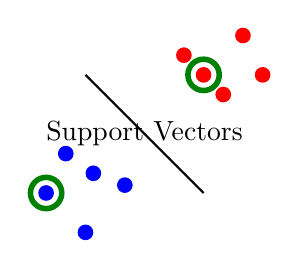
\begin{tikzpicture}[scale=0.5]
				% Draw classes
				\node[circle, fill=blue, inner sep=2pt] (a) at (0,1) {};
				\node[circle, fill=blue, inner sep=2pt] (b) at (1,0) {};
				\node[circle, fill=blue, inner sep=2pt] (c) at (1.2,1.5) {};
				\node[circle, fill=blue, inner sep=2pt] (d) at (0.5,2) {};
				\node[circle, fill=blue, inner sep=2pt] (e) at (2,1.2) {};
				\node[circle, fill=red, inner sep=2pt] (f) at (4,4) {};
				\node[circle, fill=red, inner sep=2pt] (g) at (4.5,3.5) {};
				\node[circle, fill=red, inner sep=2pt] (h) at (5,5) {};
				\node[circle, fill=red, inner sep=2pt] (i) at (3.5,4.5) {};
				\node[circle, fill=red, inner sep=2pt] (j) at (5.5,4) {};
				% Draw boundary
				\draw[thick] (1,4) -- (4,1);
				% Mark support vectors
				\node[circle, draw=green, line width=2pt, inner sep=4pt] at (0,1) {};
				\node[circle, draw=green, line width=2pt, inner sep=4pt] at (4,4) {};
				\node at (2.5,2.5) {Support Vectors};
			\end{tikzpicture}
		\end{center}
		
		\textcolor{red}{\textbf{Exam Trap:}} Only \textcolor{blue}{support vectors} influence the boundary!
	\end{frame}
	
	\begin{frame}{SVM - Soft Margin}
		\fontsize{6.5}{7.5}\selectfont
		\textcolor{blue}{\textbf{Soft Margin SVM - Handling Non-Separable Data}}
		
		\textbf{The Problem:}
		\begin{itemize}
			\item Real data is often \textcolor{red}{not perfectly separable}
			\item Hard margin SVM \textcolor{red}{fails} on overlapping data
		\end{itemize}
		
		\textbf{Soft Margin Solution:}
		\begin{itemize}
			\item Allow some points to be \textcolor{blue}{misclassified}
			\item Or allow points to fall \textcolor{blue}{inside the margin}
			\item Introduce a \textcolor{blue}{penalty} for misclassifications
		\end{itemize}
		
		\textbf{Hinge Loss:}
		\[
		L(y, f(x)) = \max(0, 1 - y f(x))
		\]
		
		\textbf{SVM Objective with Soft Margin:}
		\[
		\min_{w} \frac{1}{N}\sum_{j=1}^N \max(0, 1 - y_j(w_0 + w^T x_j)) + \frac{\lambda}{2}|w|^2
		\]
		
		\textbf{Parameter $\lambda$ (or $C$):}
		\begin{itemize}
			\item $\lambda$ large $\rightarrow$ \textcolor{blue}{Wider margin}, more misclassifications
			\item $\lambda$ small $\rightarrow$ \textcolor{blue}{Narrower margin}, fewer misclassifications
		\end{itemize}
		
		\textcolor{red}{\textbf{Exam Trap:}} $\lambda$ controls the \textcolor{blue}{trade-off} between margin width and misclassification penalty!
	\end{frame}
	
	\begin{frame}{SVM - Kernel Trick}
		\fontsize{6.5}{7.5}\selectfont
		\textcolor{blue}{\textbf{The Kernel Trick - SVM's Secret Weapon}}
		
		\textbf{The Problem:}
		\begin{itemize}
			\item Some data is \textcolor{red}{not linearly separable} in original space
			\item Example: Concentric circles - no straight line can separate them
		\end{itemize}
		
		\textbf{The Solution:}
		\begin{itemize}
			\item Project data to a \textcolor{blue}{higher-dimensional space}
			\item It may become \textcolor{blue}{linearly separable} there
			\item Example: 2D circles $\rightarrow$ 3D linear separator
		\end{itemize}
		
		\textbf{The "Trick":}
		\begin{itemize}
			\item SVM doesn't need the projected coordinates!
			\item Only needs the \textcolor{blue}{kernel function}
			\item Kernel computes dot products in the high-dimensional space
		\end{itemize}
		
		\textbf{Common Kernels:}
		\begin{enumerate}
			\item \textcolor{blue}{Linear:} $K(x, x') = x^T x'$
			\item \textcolor{blue}{Polynomial:} $K(x, x') = (x^T x' + 1)^d$
			\item \textcolor{blue}{RBF:} $K(x, x') = \exp(-\gamma \|x - x'\|^2)$
		\end{enumerate}
		
		\textcolor{red}{\textbf{Exam Trap:}} The kernel trick enables \textcolor{blue}{non-linear} classification without explicit high-dimensional computation!
	\end{frame}
	
	\begin{frame}{SVM - RBF Kernel}
		\fontsize{6.5}{7.5}\selectfont
		\textcolor{blue}{\textbf{RBF Kernel - The Most Popular Choice}}
		
		\textbf{Formula:}
		\[
		K(x, x') = \exp(-\gamma \|x - x'\|^2)
		\]
		
		\textbf{Parameter $\gamma$:}
		\begin{itemize}
			\item Controls the \textcolor{blue}{influence radius} of each training point
			\item Large $\gamma$ $\rightarrow$ \textcolor{blue}{Small influence radius}
			\begin{itemize}
				\item Each point affects only nearby points
				\item Complex, wiggly decision boundary
				\item \textcolor{red}{Risk of overfitting}
			\end{itemize}
			\item Small $\gamma$ $\rightarrow$ \textcolor{blue}{Large influence radius}
			\begin{itemize}
				\item Each point affects many points
				\item Smooth, simple decision boundary
				\item \textcolor{red}{Risk of underfitting}
			\end{itemize}
		\end{itemize}
		
		\textbf{Intuition:}
		\begin{itemize}
			\item $\gamma$ controls the \textcolor{blue}{smoothness} of the decision boundary
			\item Think of it as the \textcolor{blue}{"radius of influence"}
		\end{itemize}
		
		\textbf{Tuning $\gamma$:}
		\begin{enumerate}
			\item Try multiple $\gamma$ values (e.g., 0.001, 0.01, 0.1, 1, 10)
			\item Use \textcolor{blue}{cross-validation} to select best
			\item Combine with $C$ tuning
		\end{enumerate}
		
		\textcolor{red}{\textbf{Exam Trap:}} $\gamma$ is NOT the same as $C$ - they control different aspects of the model!
	\end{frame}
	
	\begin{frame}{SVM - Grid Search for Hyperparameters}
		\fontsize{6.5}{7.5}\selectfont
		\textcolor{blue}{\textbf{SVM Hyperparameter Tuning - Grid Search}}
		
		\textbf{Why Tune?}
		\begin{itemize}
			\item SVM performance is \textcolor{blue}{highly sensitive} to parameters
			\item Poor choice $\rightarrow$ \textcolor{red}{Poor performance}
		\end{itemize}
		
		\textbf{Key Parameters to Tune:}
		\begin{enumerate}
			\item \textcolor{blue}{$C$ (or $\lambda$)}: Soft margin penalty
			\item \textcolor{blue}{$\gamma$ (RBF)}: Kernel influence radius
			\item \textcolor{blue}{$d$ (Polynomial)}: Degree of polynomial
		\end{enumerate}
		
		\textbf{Grid Search Process:}
		\begin{enumerate}
			\item Define grid: $C \in [0.1, 1, 10, 100]$, $\gamma \in [0.01, 0.1, 1, 10]$
			\item For each combination:
			\begin{itemize}
				\item Train SVM
				\item Evaluate via cross-validation
			\end{itemize}
			\item Select combination with \textcolor{blue}{lowest validation error}
		\end{enumerate}
		
		\textbf{Example Grid:}
		\begin{tabular}{|c|c|c|}
			\hline
			\textbf{$C$} & \textbf{$\gamma$} & \textbf{Validation Accuracy} \\
			\hline
			0.1 & 0.01 & 0.85 \\
			\hline
			1 & 0.1 & 0.88 \\
			\hline
			10 & 1 & 0.87 \\
			\hline
			100 & 10 & 0.82 \\
			\hline
		\end{tabular}
		
		\textcolor{red}{\textbf{Exam Trap:}} \textcolor{blue}{Always} tune hyperparameters; defaults are rarely optimal!
	\end{frame}
	
	\begin{frame}{SVM - Advantages and Disadvantages}
		\fontsize{6.5}{7.5}\selectfont
		\textcolor{blue}{\textbf{SVM - Summary of Pros and Cons}}
		
		\textbf{Advantages:}
		\begin{enumerate}
			\item \textcolor{green}{Effective in high-dimensional spaces}
			\item \textcolor{green}{Memory efficient} (uses support vectors only)
			\item \textcolor{green}{Versatile} through kernel trick
			\item \textcolor{green}{Robust to overfitting} (margin maximization)
			\item \textcolor{green}{Theoretically well-founded}
		\end{enumerate}
		
		\textbf{Disadvantages:}
		\begin{enumerate}
			\item \textcolor{red}{Computationally expensive} for large datasets ($O(N^2)$-$O(N^3)$)
			\item \textcolor{red}{Does not directly provide probability estimates}
			\item \textcolor{red}{Sensitive to hyperparameter tuning}
			\item \textcolor{red}{Less interpretable with non-linear kernels}
			\item \textcolor{red}{Performance degrades with noise/overlapping classes}
		\end{enumerate}
		
		\textbf{When to Use SVM:}
		\begin{itemize}
			\item Medium-sized datasets
			\item High-dimensional problems
			\item When accuracy is critical
			\item When you have time for careful tuning
		\end{itemize}
		
		\textcolor{red}{\textbf{Exam Trap:}} SVM is \textcolor{blue}{powerful but requires} careful tuning and is not for massive datasets!
	\end{frame}
	
	% ============================================================
	% SECTION 4: NEURAL NETWORKS - Slides 61-85
	% ============================================================
	
	\begin{frame}{Neural Networks - Introduction}
		\fontsize{6.5}{7.5}\selectfont
		\textcolor{blue}{\textbf{Neural Networks - The Building Blocks}}
		
		\textbf{What are Neural Networks?}
		\begin{itemize}
			\item Inspired by the \textcolor{blue}{human brain}
			\item Composed of \textcolor{blue}{neurons} (nodes) organized in layers
			\item \textcolor{blue}{Feedforward} networks (MLP) are most common
		\end{itemize}
		
		\textbf{Basic Architecture:}
		
		\begin{center}
			\resizebox{0.65\textwidth}{!}{%
				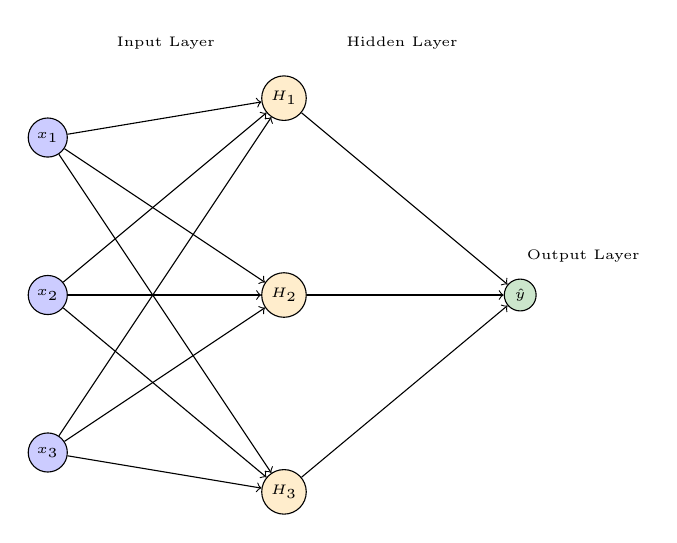
\begin{tikzpicture}[every node/.style={font=\tiny}]
					% Input layer
					\node[circle, draw, fill=blue!20, inner sep=2pt] (i1) at (0,2) {$x_1$};
					\node[circle, draw, fill=blue!20, inner sep=2pt] (i2) at (0,0) {$x_2$};
					\node[circle, draw, fill=blue!20, inner sep=2pt] (i3) at (0,-2) {$x_3$};
					% Hidden layer
					\node[circle, draw, fill=orange!20, inner sep=2pt] (h1) at (3,2.5) {$H_1$};
					\node[circle, draw, fill=orange!20, inner sep=2pt] (h2) at (3,0) {$H_2$};
					\node[circle, draw, fill=orange!20, inner sep=2pt] (h3) at (3,-2.5) {$H_3$};
					% Output layer
					\node[circle, draw, fill=green!20, inner sep=2pt] (o1) at (6,0) {$\hat{y}$};
					% Connections
					\draw[->] (i1) -- (h1);
					\draw[->] (i1) -- (h2);
					\draw[->] (i1) -- (h3);
					\draw[->] (i2) -- (h1);
					\draw[->] (i2) -- (h2);
					\draw[->] (i2) -- (h3);
					\draw[->] (i3) -- (h1);
					\draw[->] (i3) -- (h2);
					\draw[->] (i3) -- (h3);
					\draw[->] (h1) -- (o1);
					\draw[->] (h2) -- (o1);
					\draw[->] (h3) -- (o1);
					\node at (1.5,3.2) {Input Layer};
					\node at (4.5,3.2) {Hidden Layer};
					\node at (6.8,0.5) {Output Layer};
				\end{tikzpicture}%
			}
		\end{center}
		
		\textbf{Key Components:}
		\begin{enumerate}
			\item \textcolor{blue}{Weights}: Connections between neurons
			\item \textcolor{blue}{Activation Functions}: Non-linear transformations
			\item \textcolor{blue}{Bias}: Intercept term for each neuron
		\end{enumerate}
	\end{frame}
	
	\begin{frame}{Neural Networks - How Neurons Work}
		\fontsize{6.5}{7.5}\selectfont
		\textcolor{blue}{\textbf{Neuron Computation - Step by Step}}
		
		\textbf{Step 1: Weighted Sum}
		\[
		z = \sum_{i=1}^m w_i x_i + b
		\]
		where:
		\begin{itemize}
			\item $w_i$ = weights
			\item $x_i$ = inputs
			\item $b$ = bias term
		\end{itemize}
		
		\textbf{Step 2: Activation Function}
		\[
		h = f(z)
		\]
		where $f$ is a non-linear function
		
		\textbf{Example - Hidden Neuron Calculation:}
		\begin{itemize}
			\item Inputs: $x_1 = 0.6, x_2 = -0.4, x_3 = 0.3, x_4 = -0.2$
			\item Weights: $w_1 = 0.15, w_2 = -0.4, w_3 = -0.3, w_4 = 0.2$
			\item Bias: $b = 0.7$
		\end{itemize}
		
		\[
		z = 0.15(0.6) + (-0.4)(-0.4) + (-0.3)(0.3) + 0.2(-0.2) + 0.7 = 0.82
		\]
		\[
		h = \text{ReLU}(0.82) = 0.82
		\]
		
		\textbf{Key Insight:}
		\begin{itemize}
			\item Without non-linear activation, the network is just \textcolor{red}{linear regression}
			\item Activation functions enable \textcolor{blue}{complex, non-linear} learning
		\end{itemize}
	\end{frame}
	
	\begin{frame}{Neural Networks - Activation Functions}
		\fontsize{6.5}{7.5}\selectfont
		\textcolor{blue}{\textbf{Common Activation Functions}}
		
		\textbf{Sigmoid (Logistic):}
		\[
		f(z) = \frac{1}{1 + e^{-z}}
		\]
		\begin{itemize}
			\item Output: $(0, 1)$
			\item Use: Binary classification output layer
			\item \textcolor{red}{Vanishing gradient problem}
		\end{itemize}
		
		\textbf{ReLU (Rectified Linear Unit):}
		\[
		f(z) = \max(0, z)
		\]
		\begin{itemize}
			\item Output: $[0, \infty)$
			\item Use: \textcolor{blue}{Most common} for hidden layers
			\item \textcolor{green}{Efficient, helps with vanishing gradients}
			\item \textcolor{red}{Dying ReLU problem}
		\end{itemize}
		
		\textbf{Leaky ReLU:}
		\[
		f(z) = \begin{cases} 0.01z & z < 0 \\ z & z \geq 0 \end{cases}
		\]
		\begin{itemize}
			\item Fixes dying ReLU
			\item Small negative slope for $z < 0$
		\end{itemize}
		
		\textbf{Tanh:}
		\[
		f(z) = \frac{e^{2z} - 1}{e^{2z} + 1}
		\]
		\begin{itemize}
			\item Output: $(-1, 1)$
			\item Use: Recurrent neural networks
			\item \textcolor{red}{Vanishing gradient}
		\end{itemize}
		
		\textbf{Softmax:}
		\[
		f(z_i) = \frac{e^{z_i}}{\sum_{j=1}^K e^{z_j}}
		\]
		\begin{itemize}
			\item Output: Probabilities summing to 1
			\item Use: Multi-class classification output
		\end{itemize}
	\end{frame}
	
	\begin{frame}{Neural Networks - Backpropagation}
		\fontsize{6.5}{7.5}\selectfont
		\textcolor{blue}{\textbf{How Neural Networks Learn - Backpropagation}}
		
		\textbf{The Training Process:}
		
		\textbf{Step 1: Forward Pass}
		\begin{enumerate}
			\item Input $\rightarrow$ Hidden Layer $\rightarrow$ Output
			\item Calculate prediction $\hat{y}$
		\end{enumerate}
		
		\textbf{Step 2: Calculate Loss}
		\[
		L = \frac{1}{N}\sum_{i=1}^N (y_i - \hat{y}_i)^2
		\]
		or other loss function
		
		\textbf{Step 3: Backward Pass}
		\begin{enumerate}
			\item Compute gradient of loss with respect to each weight
			\item Use the \textcolor{blue}{chain rule} from calculus
			\item Propagate errors backward through the network
		\end{enumerate}
		
		\textbf{Step 4: Update Weights}
		\[
		w_{new} = w_{old} - \eta \frac{\partial L}{\partial w}
		\]
		where $\eta$ is the \textcolor{blue}{learning rate}
		
		\textbf{Repeat:}
		\begin{itemize}
			\item For many \textcolor{blue}{epochs} (passes through data)
			\item Until convergence or early stopping
		\end{itemize}
		
		\textcolor{red}{\textbf{Exam Trap:}} Backpropagation is just \textcolor{blue}{gradient descent} applied to neural networks!
	\end{frame}
	
	\begin{frame}{Neural Networks - Overfitting}
		\fontsize{6.5}{7.5}\selectfont
		\textcolor{blue}{\textbf{Overfitting in Neural Networks}}
		
		\textbf{Why Neural Networks Overfit:}
		\begin{itemize}
			\item \textcolor{blue}{Too many parameters} (weights)
			\item Can \textcolor{red}{memorize} training data
			\item Learns \textcolor{red}{noise and artifacts}
		\end{itemize}
		
		\textbf{Signs of Overfitting:}
		\begin{enumerate}
			\item Training error $\downarrow$, Validation error $\uparrow$
			\item Different predictions from different training runs
			\item Extremely high training accuracy, poor test accuracy
		\end{enumerate}
		
		\textbf{Prevention Techniques:}
		
		\begin{tabular}{|p{4cm}|p{4cm}|}
			\hline
			\textbf{Technique} & \textbf{How It Works} \\
			\hline
			L2 Regularization & Penalty on large weights \\
			\hline
			Dropout & Randomly drop neurons during training \\
			\hline
			Early Stopping & Stop when validation error increases \\
			\hline
			More Data & More training examples \\
			\hline
			Data Augmentation & Create variations of training data \\
			\hline
			Smaller Network & Fewer parameters \\
			\hline
		\end{tabular}
		
		\textbf{L2 Regularization:}
		\[
		L_{new} = L_{old} + \lambda \sum w_i^2
		\]
		
		\textcolor{red}{\textbf{Exam Trap:}} \textcolor{blue}{Multiple techniques} together are more effective than any single one!
	\end{frame}
	
	\begin{frame}{Neural Networks - Dropout}
		\fontsize{6.5}{7.5}\selectfont
		\textcolor{blue}{\textbf{Dropout - Ensemble in a Single Network}}
		
		\textbf{What is Dropout?}
		\begin{itemize}
			\item Randomly \textcolor{blue}{drop} neurons during training
			\item Each neuron has probability $p$ of being dropped
			\item Common $p = 0.5$ (50\% dropout)
		\end{itemize}
		
		\textbf{How It Works:}
		\begin{enumerate}
			\item For each training iteration:
			\begin{itemize}
				\item Randomly select neurons to \textcolor{blue}{drop}
				\item Dropped neurons output 0
				\item Only remaining neurons participate
			\end{itemize}
			\item Different network architecture each iteration
			\item At test time: \textcolor{blue}{All} neurons used (scaled)
		\end{enumerate}
		
		\textbf{Why It Works:}
		\begin{itemize}
			\item Prevents \textcolor{blue}{co-adaptation} of neurons
			\item Forces network to learn \textcolor{blue}{robust} features
			\item Acts as an \textcolor{blue}{ensemble} of many networks
		\end{itemize}
		
		\textbf{Example:}
		\begin{itemize}
			\item Network with 100 neurons, dropout $p = 0.5$
			\item Each iteration uses \textcolor{blue}{about 50} neurons
			\item Over training, \textcolor{blue}{many} different sub-networks
			\item Final model averages all sub-networks
		\end{itemize}
		
		\textcolor{red}{\textbf{Exam Trap:}} Dropout is applied \textcolor{blue}{only during training}, not at test time!
	\end{frame}
	
	\begin{frame}{Neural Networks - Early Stopping}
		\fontsize{6.5}{7.5}\selectfont
		\textcolor{blue}{\textbf{Early Stopping - The Simplest Regularization}}
		
		\textbf{The Concept:}
		\begin{itemize}
			\item Monitor \textcolor{blue}{validation error} during training
			\item Stop when validation error \textcolor{red}{starts to increase}
			\item Even if training error continues to decrease
		\end{itemize}
		
		\textbf{Visual Representation:}
		\begin{center}
			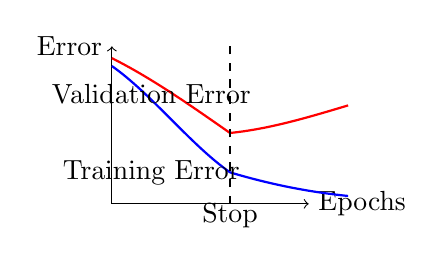
\begin{tikzpicture}[scale=0.5]
				\draw[->] (0,0) -- (5,0) node[right] {Epochs};
				\draw[->] (0,0) -- (0,4) node[left] {Error};
				\draw[blue, thick] (0,3.5) .. controls (1,2.8) and (2,1.5) .. (3,0.8) .. controls (4,0.5) and (5,0.3) .. (6,0.2);
				\draw[red, thick] (0,3.7) .. controls (1,3.2) and (2,2.5) .. (3,1.8) .. controls (4,1.9) and (5,2.2) .. (6,2.5);
				\draw[dashed, thick] (3,0) -- (3,4);
				\node at (3,-0.3) {Stop};
				\node at (1,0.8) {Training Error};
				\node at (1,2.8) {Validation Error};
			\end{tikzpicture}
		\end{center}
		
		\textbf{Why It Works:}
		\begin{itemize}
			\item Early training: Learning \textcolor{blue}{general patterns}
			\item Late training: Learning \textcolor{red}{noise}
			\item Stop at optimal point of \textcolor{blue}{generalization}
		\end{itemize}
		
		\textbf{Practical Implementation:}
		\begin{enumerate}
			\item Hold out 20-30\% of data as validation set
			\item Train network, monitor validation error
			\item Stop when validation error hasn't improved for $k$ epochs
			\item Use model from \textcolor{blue}{best} epoch
		\end{enumerate}
	\end{frame}
	
	\begin{frame}{Neural Networks - CNNs}
		\fontsize{6.5}{7.5}\selectfont
		\textcolor{blue}{\textbf{Convolutional Neural Networks (CNNs)}}
		
		\textbf{What CNNs Are Designed For:}
		\begin{itemize}
			\item Data with \textcolor{blue}{grid-like topology}
			\item \textcolor{blue}{Images} (2D grid of pixels)
			\item Also: Text (1D grid), time series
		\end{itemize}
		
		\textbf{Key Innovation - Convolution:}
		\begin{itemize}
			\item Uses \textcolor{blue}{filters (kernels)} that slide across input
			\item Each filter detects a specific pattern
			\item Results in a \textcolor{blue}{feature map}
		\end{itemize}
		
		\textbf{Advantages of Convolution:}
		\begin{enumerate}
			\item \textcolor{blue}{Parameter Sharing}: Same filter applied everywhere
			\item \textcolor{blue}{Translation Invariance}: Pattern recognized regardless of location
			\item \textcolor{blue}{Sparse Connections}: Each output depends on small local region
		\end{enumerate}
		
		\textbf{CNN Architecture:}
		\begin{center}
			\resizebox{0.7\textwidth}{!}{%
				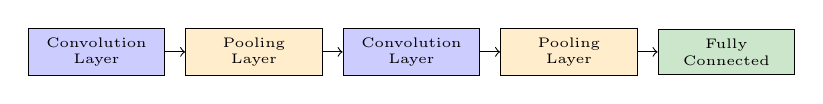
\begin{tikzpicture}[every node/.style={font=\tiny}]
					\node[draw, rectangle, fill=blue!20, text width=1.5cm, align=center] (conv1) {Convolution\\Layer};
					\node[draw, rectangle, fill=orange!20, text width=1.5cm, align=center] (pool1) [right of=conv1, xshift=1cm] {Pooling\\Layer};
					\node[draw, rectangle, fill=blue!20, text width=1.5cm, align=center] (conv2) [right of=pool1, xshift=1cm] {Convolution\\Layer};
					\node[draw, rectangle, fill=orange!20, text width=1.5cm, align=center] (pool2) [right of=conv2, xshift=1cm] {Pooling\\Layer};
					\node[draw, rectangle, fill=green!20, text width=1.5cm, align=center] (fc) [right of=pool2, xshift=1cm] {Fully\\Connected};
					\draw[->] (conv1) -- (pool1);
					\draw[->] (pool1) -- (conv2);
					\draw[->] (conv2) -- (pool2);
					\draw[->] (pool2) -- (fc);
				\end{tikzpicture}%
			}
		\end{center}
		
		\textcolor{red}{\textbf{Exam Trap:}} CNNs are \textcolor{blue}{not} just for images; they work on any grid-like data!
	\end{frame}
	
	\begin{frame}{Neural Networks - CNN Components}
		\fontsize{6.5}{7.5}\selectfont
		\textcolor{blue}{\textbf{CNN Components - Detailed Explanation}}
		
		\textbf{Convolutional Layer:}
		\begin{itemize}
			\item Applies filters to input
			\item Each filter creates a \textcolor{blue}{feature map}
			\item Number of filters $\rightarrow$ number of feature maps
		\end{itemize}
		
		\textbf{Filter (Kernel) Example:}
		\begin{itemize}
			\item 3x3 kernel slides over 4x4 image
			\item Each position produces one value
			\item Result: 2x2 feature map
		\end{itemize}
		
		\textbf{Pooling Layer:}
		\begin{itemize}
			\item Reduces \textcolor{blue}{spatial dimensions}
			\item Common: Max pooling (take max value in window)
			\item Also: Average pooling
			\item Increases \textcolor{blue}{translation invariance}
		\end{itemize}
		
		\textbf{Pooling Example:}
		\begin{itemize}
			\item 2x2 max pooling on 4x4 feature map
			\item Result: 2x2 feature map
			\item Takes maximum value from each 2x2 block
		\end{itemize}
		
		\textbf{Fully Connected Layers:}
		\begin{itemize}
			\item At the end of the network
			\item Use high-level features for classification
			\item Standard neural network layers
		\end{itemize}
		
		\textcolor{red}{\textbf{Exam Trap:}} Pooling \textcolor{blue}{reduces} dimensions, convolution \textcolor{blue}{preserves or changes} dimensions based on padding!
	\end{frame}
	
	\begin{frame}{Neural Networks - RNNs}
		\fontsize{6.5}{7.5}\selectfont
		\textcolor{blue}{\textbf{Recurrent Neural Networks (RNNs)}}
		
		\textbf{What Makes RNNs Special:}
		\begin{itemize}
			\item Have \textcolor{blue}{memory}
			\item Process \textcolor{blue}{sequential} data
			\item Each output depends on previous inputs
		\end{itemize}
		
		\textbf{Common Applications:}
		\begin{enumerate}
			\item Time series forecasting
			\item Natural language processing
			\item Speech recognition
			\item Text generation
		\end{enumerate}
		
		\textbf{RNN Structure:}
		\begin{center}
			\resizebox{0.55\textwidth}{!}{%
				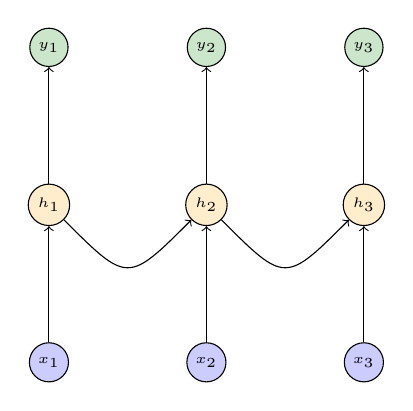
\begin{tikzpicture}[every node/.style={font=\tiny}]
					\node[circle, draw, fill=blue!20, inner sep=2pt] (x1) at (0,0) {$x_1$};
					\node[circle, draw, fill=blue!20, inner sep=2pt] (x2) at (2,0) {$x_2$};
					\node[circle, draw, fill=blue!20, inner sep=2pt] (x3) at (4,0) {$x_3$};
					\node[circle, draw, fill=orange!20, inner sep=2pt] (h1) at (0,2) {$h_1$};
					\node[circle, draw, fill=orange!20, inner sep=2pt] (h2) at (2,2) {$h_2$};
					\node[circle, draw, fill=orange!20, inner sep=2pt] (h3) at (4,2) {$h_3$};
					\node[circle, draw, fill=green!20, inner sep=2pt] (y1) at (0,4) {$y_1$};
					\node[circle, draw, fill=green!20, inner sep=2pt] (y2) at (2,4) {$y_2$};
					\node[circle, draw, fill=green!20, inner sep=2pt] (y3) at (4,4) {$y_3$};
					\draw[->] (x1) -- (h1);
					\draw[->] (x2) -- (h2);
					\draw[->] (x3) -- (h3);
					\draw[->] (h1) -- (y1);
					\draw[->] (h2) -- (y2);
					\draw[->] (h3) -- (y3);
					\draw[->] (h1) .. controls (1,1) .. (h2);
					\draw[->] (h2) .. controls (3,1) .. (h3);
				\end{tikzpicture}%
			}
		\end{center}
		
		\textbf{Limitation:}
		\begin{itemize}
			\item \textcolor{red}{Vanishing gradients} in long sequences
			\item Cannot learn long-term dependencies
		\end{itemize}
		
		\textcolor{red}{\textbf{Exam Trap:}} RNNs are for \textcolor{blue}{sequential} data - don't use them on non-sequential data!
	\end{frame}
	
	\begin{frame}{Neural Networks - LSTMs}
		\fontsize{6.5}{7.5}\selectfont
		\textcolor{blue}{\textbf{Long Short-Term Memory (LSTM) Networks}}
		
		\textbf{The Problem with Basic RNNs:}
		\begin{itemize}
			\item Cannot remember information for \textcolor{red}{long periods}
			\item \textcolor{red}{Vanishing gradients} in long sequences
		\end{itemize}
		
		\textbf{How LSTMs Solve This:}
		\begin{itemize}
			\item Add a \textcolor{blue}{memory cell}
			\item Use \textcolor{blue}{gates} to control information flow
			\item Can keep information for \textcolor{green}{long periods}
		\end{itemize}
		
		\textbf{The Three Gates:}
		
		\begin{tabular}{|p{3cm}|p{5cm}|}
			\hline
			\textbf{Gate} & \textbf{Function} \\
			\hline
			Forget Gate & Decides what to \textcolor{red}{discard} from memory \\
			\hline
			Input Gate & Decides what \textcolor{blue}{new information} to store \\
			\hline
			Output Gate & Decides what to \textcolor{blue}{output} from memory \\
			\hline
		\end{tabular}
		
		\textbf{Memory Cell:}
		\begin{itemize}
			\item Stores information over time
			\item Can hold information for \textcolor{blue}{thousands of steps}
			\item Prevents vanishing gradients
		\end{itemize}
		
		\textbf{Why LSTMs Are Popular:}
		\begin{enumerate}
			\item \textcolor{green}{Handle long sequences well}
			\item \textcolor{green}{State-of-the-art on many tasks}
			\item \textcolor{green}{Used in transformers and language models}
		\end{enumerate}
		
		\textcolor{red}{\textbf{Exam Trap:}} LSTMs are an \textcolor{blue}{evolution} of RNNs, not a completely different architecture!
	\end{frame}
	
	% ============================================================
	% SECTION 5: AUTOENCODERS - Slides 86-100
	% ============================================================
	
	\begin{frame}{Autoencoders - Introduction}
		\fontsize{6.5}{7.5}\selectfont
		\textcolor{blue}{\textbf{Autoencoders - Overview}}
		
		\textbf{What is an Autoencoder?}
		\begin{itemize}
			\item \textcolor{blue}{Unsupervised} neural network
			\item Learns to \textcolor{blue}{compress} and \textcolor{blue}{reconstruct} data
			\item Uses \textcolor{blue}{no labels} - pure unsupervised learning
		\end{itemize}
		
		\textbf{Architecture:}
		
		\begin{center}
			\resizebox{0.7\textwidth}{!}{%
				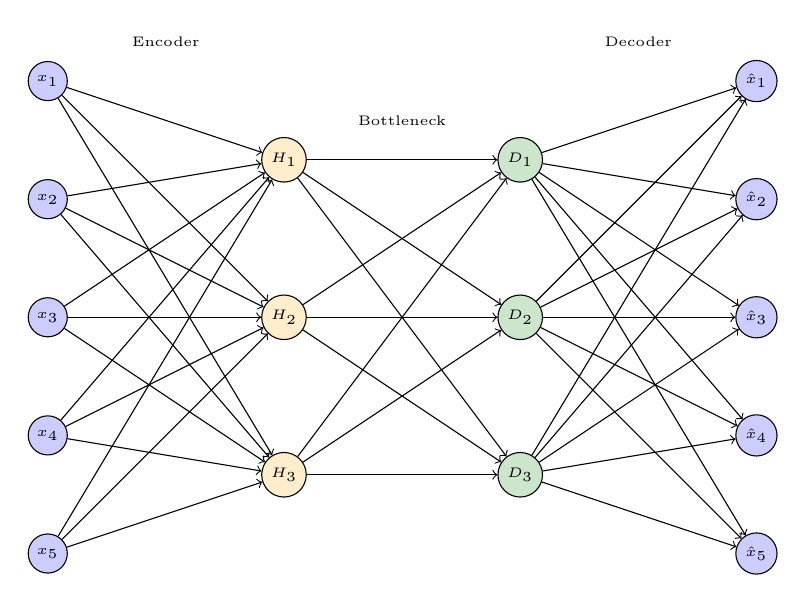
\begin{tikzpicture}[every node/.style={font=\tiny}]
					% Input
					\node[circle, draw, fill=blue!20, inner sep=2pt] (i1) at (0,3) {$x_1$};
					\node[circle, draw, fill=blue!20, inner sep=2pt] (i2) at (0,1.5) {$x_2$};
					\node[circle, draw, fill=blue!20, inner sep=2pt] (i3) at (0,0) {$x_3$};
					\node[circle, draw, fill=blue!20, inner sep=2pt] (i4) at (0,-1.5) {$x_4$};
					\node[circle, draw, fill=blue!20, inner sep=2pt] (i5) at (0,-3) {$x_5$};
					% Encoder hidden
					\node[circle, draw, fill=orange!20, inner sep=2pt] (h1) at (3,2) {$H_1$};
					\node[circle, draw, fill=orange!20, inner sep=2pt] (h2) at (3,0) {$H_2$};
					\node[circle, draw, fill=orange!20, inner sep=2pt] (h3) at (3,-2) {$H_3$};
					% Decoder hidden
					\node[circle, draw, fill=green!20, inner sep=2pt] (d1) at (6,2) {$D_1$};
					\node[circle, draw, fill=green!20, inner sep=2pt] (d2) at (6,0) {$D_2$};
					\node[circle, draw, fill=green!20, inner sep=2pt] (d3) at (6,-2) {$D_3$};
					% Output
					\node[circle, draw, fill=blue!20, inner sep=2pt] (o1) at (9,3) {$\hat{x}_1$};
					\node[circle, draw, fill=blue!20, inner sep=2pt] (o2) at (9,1.5) {$\hat{x}_2$};
					\node[circle, draw, fill=blue!20, inner sep=2pt] (o3) at (9,0) {$\hat{x}_3$};
					\node[circle, draw, fill=blue!20, inner sep=2pt] (o4) at (9,-1.5) {$\hat{x}_4$};
					\node[circle, draw, fill=blue!20, inner sep=2pt] (o5) at (9,-3) {$\hat{x}_5$};
					% Connections
					\foreach \i in {1,...,5}
					\foreach \j in {1,...,3}
					\draw[->] (i\i) -- (h\j);
					\foreach \i in {1,...,3}
					\foreach \j in {1,...,3}
					\draw[->] (h\i) -- (d\j);
					\foreach \i in {1,...,3}
					\foreach \j in {1,...,5}
					\draw[->] (d\i) -- (o\j);
					% Labels
					\node at (1.5,3.5) {Encoder};
					\node at (4.5,2.5) {Bottleneck};
					\node at (7.5,3.5) {Decoder};
				\end{tikzpicture}%
			}
		\end{center}
		
		\textbf{Key Components:}
		\begin{enumerate}
			\item \textcolor{blue}{Encoder}: Compresses input to latent representation
			\item \textcolor{blue}{Bottleneck}: Lower-dimensional hidden layer
			\item \textcolor{blue}{Decoder}: Reconstructs from latent representation
		\end{enumerate}
	\end{frame}
	
	\begin{frame}{Autoencoders - How They Learn}
		\fontsize{6.5}{7.5}\selectfont
		\textcolor{blue}{\textbf{How Autoencoders Learn - The Training Process}}
		
		\textbf{Training Objective:}
		\begin{itemize}
			\item Minimize \textcolor{blue}{reconstruction error}
			\item Input $\approx$ Output
		\end{itemize}
		
		\textbf{Loss Function - Mean Squared Error:}
		\[
		L = \frac{1}{mN} \sum_{j=1}^m \sum_{i=1}^N (x_{ij} - \hat{x}_{ij})^2
		\]
		
		\textbf{The Bottleneck Effect:}
		\begin{itemize}
			\item Hidden layer has \textcolor{blue}{fewer neurons} than input
			\item Forces \textcolor{blue}{compression}
			\item Network must learn \textcolor{blue}{important features}
		\end{itemize}
		
		\textbf{Example:}
		\begin{itemize}
			\item Input: 100 features
			\item Bottleneck: 10 neurons
			\item Network learns to represent 100 features with just 10 numbers
			\item Reconstruction will lose some detail
			\item But \textcolor{blue}{important patterns are preserved}
		\end{itemize}
		
		\textbf{What the Network Learns:}
		\begin{enumerate}
			\item \textcolor{blue}{Most important features}
			\item \textcolor{blue}{Relationships between features}
			\item \textcolor{blue}{Dimensionality reduction}
		\end{enumerate}
	\end{frame}
	
	\begin{frame}{Autoencoders - Linear vs Non-Linear}
		\fontsize{6.5}{7.5}\selectfont
		\textcolor{blue}{\textbf{Linear Autoencoders vs Non-Linear Autoencoders}}
		
		\textbf{Linear Autoencoder:}
		\begin{itemize}
			\item Uses \textcolor{blue}{only linear} activation functions
			\item Equivalent to \textcolor{blue}{PCA}
			\item Cannot capture non-linear relationships
		\end{itemize}
		
		\textbf{Non-Linear Autoencoder:}
		\begin{itemize}
			\item Uses \textcolor{blue}{non-linear} activation functions (ReLU, sigmoid)
			\item Can capture \textcolor{blue}{complex} relationships
			\item More powerful than PCA
		\end{itemize}
		
		\textbf{Comparison Table:}
		
		\begin{tabular}{|p{4cm}|p{4cm}|}
			\hline
			\textbf{Linear Autoencoder} & \textbf{Non-Linear Autoencoder} \\
			\hline
			Equivalent to PCA & More powerful than PCA \\
			\hline
			No non-linearity & Non-linear activation functions \\
			\hline
			Unique solution & Many possible solutions \\
			\hline
			Fast training & Slower training \\
			\hline
			Less flexible & More flexible \\
			\hline
		\end{tabular}
		
		\textbf{When to Use Which:}
		\begin{itemize}
			\item Linear: Simple data, need speed
			\item Non-linear: Complex data, need power
		\end{itemize}
		
		\textcolor{red}{\textbf{Exam Trap:}} A linear autoencoder with one hidden layer is \textcolor{blue}{equivalent to PCA}!
	\end{frame}
	
	\begin{frame}{Autoencoders - Variants}
		\fontsize{6.5}{7.5}\selectfont
		\textcolor{blue}{\textbf{Autoencoder Variants - Specialized Versions}}
		
		\textbf{Sparse Autoencoder:}
		\begin{itemize}
			\item More hidden neurons than input
			\item But most weights are \textcolor{blue}{near zero} (sparse)
			\item Uses L1 regularization
			\item Learns \textcolor{blue}{sparse} representations
		\end{itemize}
		
		\textbf{Denoising Autoencoder:}
		\begin{itemize}
			\item Trained on \textcolor{blue}{corrupted} inputs
			\item Reconstructs \textcolor{blue}{clean} version
			\item Learns \textcolor{blue}{robust} features
			\item Great for noise removal
		\end{itemize}
		
		\textbf{Deep Autoencoder:}
		\begin{itemize}
			\item Multiple hidden layers
			\item Symmetrical architecture
			\item Captures \textcolor{blue}{hierarchical} features
			\item More powerful for complex data
		\end{itemize}
		
		\textbf{Variational Autoencoder (VAE):}
		\begin{itemize}
			\item Probabilistic version
			\item Learns \textcolor{blue}{latent distribution}
			\item Can \textcolor{blue}{generate} new data
			\item Used in generative AI
		\end{itemize}
		
		\textcolor{red}{\textbf{Exam Trap:}} Different variants serve \textcolor{blue}{different purposes} - choose based on the task!
	\end{frame}
	
	\begin{frame}{Autoencoders - Anomaly Detection}
		\fontsize{6.5}{7.5}\selectfont
		\textcolor{blue}{\textbf{Autoencoders for Anomaly Detection - The Risk Management Application}}
		
		\textbf{The Process:}
		\begin{enumerate}
			\item Train autoencoder on \textcolor{blue}{normal data only}
			\item The model learns to reconstruct normal patterns
			\item For new data:
			\begin{itemize}
				\item Calculate \textcolor{blue}{reconstruction error}
				\item Low error $\rightarrow$ \textcolor{green}{Normal}
				\item High error $\rightarrow$ \textcolor{red}{Anomaly}
			\end{itemize}
		\end{enumerate}
		
		\textbf{Why This Works:}
		\begin{itemize}
			\item Anomalies are \textcolor{blue}{different} from normal data
			\item Autoencoder trained only on normal data
			\item Cannot reconstruct anomalies well
			\item High reconstruction error indicates \textcolor{red}{anomaly}
		\end{itemize}
		
		\textbf{Example - Fraud Detection:}
		\begin{itemize}
			\item Train on normal transactions
			\item Fraudulent transaction $\rightarrow$ high reconstruction error
			\item Flag for investigation
		\end{itemize}
		
		\textbf{Threshold Selection:}
		\begin{itemize}
			\item Compute reconstruction errors on validation set
			\item Set threshold at, e.g., 95th percentile
			\item Error $>$ threshold $\rightarrow$ \textcolor{red}{Anomaly}
		\end{itemize}
		
		\textcolor{red}{\textbf{Exam Trap:}} Autoencoders detect anomalies by \textcolor{blue}{high reconstruction error} - not by classification!
	\end{frame}
	
	\begin{frame}{Autoencoders - Advantages and Disadvantages}
		\fontsize{6.5}{7.5}\selectfont
		\textcolor{blue}{\textbf{Autoencoders - Summary of Pros and Cons}}
		
		\textbf{Advantages:}
		\begin{enumerate}
			\item \textcolor{green}{Unsupervised} - no labels needed
			\item \textcolor{green}{Can capture non-linear} relationships
			\item \textcolor{green}{Great for dimensionality reduction}
			\item \textcolor{green}{Excellent for anomaly detection}
			\item \textcolor{green}{Can generate new data} (VAEs)
			\item \textcolor{green}{Feature extraction} for other models
		\end{enumerate}
		
		\textbf{Disadvantages:}
		\begin{enumerate}
			\item \textcolor{red}{Can be computationally expensive} to train
			\item \textcolor{red}{Hyperparameter sensitive} (architecture, learning rate)
			\item \textcolor{red}{Not interpretable} - latent space is abstract
			\item \textcolor{red}{May not generalize} to unseen data types
			\item \textcolor{red}{Requires careful tuning} for good results
		\end{enumerate}
		
		\textbf{When to Use Autoencoders:}
		\begin{itemize}
			\item Dimensionality reduction (when PCA isn't enough)
			\item Anomaly detection (fraud, operational risk)
			\item Feature learning (pre-training for other models)
			\item Data denoising (cleaning noisy data)
		\end{itemize}
		
		\textcolor{red}{\textbf{Exam Trap:}} Autoencoders are \textcolor{blue}{powerful but require} careful design and tuning!
	\end{frame}
	
	\begin{frame}{Autoencoders - Comparison with PCA}
		\fontsize{6.5}{7.5}\selectfont
		\textcolor{blue}{\textbf{Autoencoders vs PCA - Detailed Comparison}}
		
		\textbf{Key Differences:}
		
		\begin{tabular}{|p{4cm}|p{4cm}|}
			\hline
			\textcolor{blue}{Autoencoder} & \textcolor{blue}{PCA} \\
			\hline
			Non-linear & Linear \\
			\hline
			Learns representation & Finds variance directions \\
			\hline
			Neural network & Matrix decomposition \\
			\hline
			Can be deep & Single transformation \\
			\hline
			Flexible architecture & Fixed mathematical solution \\
			\hline
			Sensitive to hyperparameters & No hyperparameters \\
			\hline
			Slower to train & Fast \\
			\hline
			Can handle complex data & Limited to linear relationships \\
			\hline
		\end{tabular}
		
		\textbf{When Autoencoders Win:}
		\begin{itemize}
			\item Data has \textcolor{blue}{non-linear} structure
			\item Need \textcolor{blue}{more compact} representation
			\item Want to learn \textcolor{blue}{features} for other tasks
		\end{itemize}
		
		\textbf{When PCA Wins:}
		\begin{itemize}
			\item Data is \textcolor{blue}{linear}
			\item Need \textcolor{blue}{fast} computation
			\item Need \textcolor{blue}{interpretable} components
			\item Need \textcolor{blue}{reproducible} results
		\end{itemize}
		
		\textcolor{red}{\textbf{Exam Trap:}} Autoencoders are \textcolor{blue}{non-linear PCA} - choose based on data complexity!
	\end{frame}
	
	\begin{frame}{Autoencoders - Treasury Yield Example}
		\fontsize{6.5}{7.5}\selectfont
		\textcolor{blue}{\textbf{Autoencoders in Practice - Treasury Yield Data}}
		
		\textbf{Dataset:}
		\begin{itemize}
			\item 8 Treasury yield series
			\item Daily changes in yields
			\item High-dimensional time series
		\end{itemize}
		
		\textbf{Goal:}
		\begin{itemize}
			\item Reduce dimensionality
			\item Capture yield curve dynamics
			\item Compare to PCA
		\end{itemize}
		
		\textbf{Results:}
		
		\begin{tabular}{|c|c|c|c|}
			\hline
			\textbf{Components} & \textbf{PCA MSE} & \textbf{Hidden Units} & \textbf{Autoencoder MSE} \\
			\hline
			1 & 0.18208 & 1 & 0.18270 \\
			\hline
			2 & 0.04965 & 2 & 0.05027 \\
			\hline
			3 & 0.01708 & 3 & 0.01740 \\
			\hline
			4 & 0.00848 & 4 & 0.00854 \\
			\hline
			5 & 0.00528 & 5 & 0.00534 \\
			\hline
			6 & 0.00295 & 6 & 0.00299 \\
			\hline
			7 & 0.00107 & 7 & 0.00113 \\
			\hline
			8 & 0.00000 & 8 & 0.00000 \\
			\hline
		\end{tabular}
		
		\textbf{Interpretation:}
		\begin{itemize}
			\item Autoencoder and PCA performed \textcolor{blue}{similarly}
			\item Linear structure dominated yield curve
			\item Autoencoder didn't provide significant improvement
			\item \textcolor{red}{Not all problems benefit from non-linearity!}
		\end{itemize}
	\end{frame}
	
	\begin{frame}{TUTORIAL SUMMARY}
		\fontsize{6.5}{7.5}\selectfont
		\textcolor{blue}{\textbf{Complete Tutorial Summary - Key Takeaways}}
		
		\textbf{Decision Trees:}
		\begin{itemize}
			\item White-box models, highly interpretable
			\item Regression (RSS) vs Classification (Entropy/Gini)
			\item Pruning prevents overfitting
			\item Ensembles (Bagging, RF, Boosting) improve accuracy
		\end{itemize}
		
		\textbf{K-Nearest Neighbors:}
		\begin{itemize}
			\item Lazy learner, no training phase
			\item Distance-based, requires feature scaling
			\item K controls bias-variance trade-off
			\item Curse of dimensionality in high dimensions
		\end{itemize}
		
		\textbf{Support Vector Machines:}
		\begin{itemize}
			\item Maximum margin classifier
			\item Support vectors define the boundary
			\item Kernel trick enables non-linear boundaries
			\item Requires careful hyperparameter tuning
		\end{itemize}
		
		\textbf{Neural Networks:}
		\begin{itemize}
			\item Universal approximators
			\item Activation functions provide non-linearity
			\item Backpropagation for training
			\item Overfitting prevention: regularization, dropout, early stopping
		\end{itemize}
		
		\textbf{Autoencoders:}
		\begin{itemize}
			\item Unsupervised dimensionality reduction
			\item Encoder-Decoder architecture
			\item Can capture non-linear relationships
			\item Anomaly detection through reconstruction error
		\end{itemize}
		
		\textcolor{red}{\textbf{Exam Success Tip:}} Understand the \textcolor{blue}{"why"} behind each algorithm, not just the \textcolor{blue}{"how"}!
	\end{frame}
	
	\begin{frame}{FINAL EXAM TIPS}
		\fontsize{6.5}{7.5}\selectfont
		\textcolor{blue}{\textbf{Top 10 Exam Traps to Remember:}}
		
		\begin{enumerate}
			\item \textcolor{red}{Trap 1:} Decision trees are \textcolor{blue}{white-box} (interpretable), not black-box
			\item \textcolor{red}{Trap 2:} Regression trees use \textcolor{blue}{RSS}; classification trees use \textcolor{blue}{Entropy/Gini}
			\item \textcolor{red}{Trap 3:} KNN \textcolor{blue}{requires feature scaling} - it's not optional!
			\item \textcolor{red}{Trap 4:} Small K in KNN $\rightarrow$ \textcolor{blue}{overfitting}; large K $\rightarrow$ \textcolor{blue}{underfitting}
			\item \textcolor{red}{Trap 5:} SVM maximizes \textcolor{blue}{margin}; support vectors are the \textcolor{blue}{closest points}
			\item \textcolor{red}{Trap 6:} Kernel trick enables \textcolor{blue}{non-linear} SVM without explicit high-dimensional computation
			\item \textcolor{red}{Trap 7:} Neural networks need \textcolor{blue}{non-linear} activation functions; linear = regression
			\item \textcolor{red}{Trap 8:} Dropout is \textcolor{blue}{only during training}, not at test time
			\item \textcolor{red}{Trap 9:} Autoencoders are \textcolor{blue}{unsupervised}; they reconstruct, not classify
			\item \textcolor{red}{Trap 10:} Linear autoencoder with one hidden layer = \textcolor{blue}{PCA}
		\end{enumerate}
		
		\textcolor{blue}{\textbf{Remember:}} The exam tests conceptual understanding, not just memorization!
	\end{frame}
	
\end{document}